\chapter{Optimisation under Uncertainty}
\label{sec:opt}

This chapter is dedicated to introducing applied optimisation and modification concepts. It commences with the mathematical problem formulation in \Autoref{sec:pf} building on the parameters presented in \Autoref{sec:model}, where objectives and constraints are categorised and complemented with an explanation of their purpose. Furthermore, a method for linear power flow approximation to enable solutions obtained from quick linear programming. Subsequently reference charging approaches are introduced in \Autoref{sec:rc} against which coordinating scheduling algorithms are held as a benchmark. These are presented and discussed in \Autoref{sec:chargecoordination} before addressing various methods of uncertainty mitigation in \Autoref{sec:uncmitigation}.

\section{Problem Formulation}
\label{sec:pf}

Following a time discretization to avoid formal representations by differential equations, constant charging powers within each time slot are assumed. Across time slots $\Delta t = 0.25$ hours, the charging rates are continuous and are denoted by the matrix of decision variables  $P^{EV}\in \mathbb{R}^{K\times T}$.

\subsection{Objectives}

The objective function is designed to find a set of schedules $P^{EV}$ which minimise the costs of charging a pool of electric vehicles in discrete time steps $\Delta t$. Primarily, it is a customer-focused objective providing an incentive for EV users to devise charging control to the aggregator. However, it may also be regarded as beneficial from a system point of view as the price forecasts mirror the expected overall demand and supply situation. With the expected electricity prices given by $\hat{\pi}_t$, the objective function $C$ is

\begin{equation}
	\label{eq:obj1}
	\min_{\{P^{EV}\}} C=\sum_{t=1}^T \sum_{k=1}^{K} \quad \hat{\pi}_t \cdot \Delta t \cdot \pev 
\end{equation}

The objective function $C$ from \Autoref{eq:obj1} can be extended to include revenues from the provision of regulation capacity subject to further constraints about the battery state of charge described in \Autoref{eq:reg_constraint}, yielding

\begin{equation}
	\label{eq:obj2}
	\min_{\{P^{EV},\omega\}} C'=\sum_{t=1}^T \sum_{k=1}^{K} \quad \hat{\pi}_t \cdot \Delta t \cdot \pev \quad - \quad \rho \cdot \eta \cdot P^{EV}_{max} \cdot \lev 
\end{equation}

where $\rho$ is the reward, in p/kW$\cdot$h for the provision of capacity available for regulation, $\eta$ denotes the discharging efficiency, and $\omega_{k,t}$ is the decision variable indicating the current provision of regulating capacity. % Positive control and feeding back electricity are not found to be promising options due to the costs in terms of battery degrada- tion and for the bidirectional power electronics. Dallinger2010a

\subsection{Constraints}

The objective function is subject to a number of constraints. These can be broadly split into constraints concerning the observation of electric vehicle technical limitations, the satisfaction of users' requirements or network-related constraints. Each of the constraints is applied for all households $k \in K$, time slots $t \in T$, and lines $\ell \in L$.

First, the charging rate is constrained by the limits of the applied charging mode. Disabling discharge capabilities of the EV battery the constraint forms as
\begin{equation}
0  \leq \pev \leq P^{EV}_{max},
\end{equation}
where due to exclusive standard single-phase connections $P^{EV}_{max} = 3.7$ kWh.

Moreover, an electric vehicle may only be scheduled to charge when it is expected to be available and plugged in. Therefore,

\begin{equation}
\left(1-\aev\right)\cdot \pev = 0 
\end{equation}

where $\aev \in \mathbb{B}$ is the parameter denoting the presumed availability of an electric vehicle at household $k$ in time slot $t$.

The primary user satisfaction constraint is charging EVs to provide an adequate driving range. Hence, starting from a vehicle's expected battery state of charge upon arrival $\hat{B}^{arr}_{k} \in [0,B_{max}]$, the charged energy over all slots $t \in T$ of the optimisation horizon under consideration of the charging efficiency $\eta=0.93$ must accumulate to a full battery state of charge $B_{max} = 30$ kWh.

\begin{equation}
\hat{B}^{arr}_{k}+\sum_{t=1}^{T} \eta \cdot \pev \cdot \Delta t = B_{max}
\end{equation}

Other target values for the battery state of charge are conceivable and may already satisfy a majority of mobility requirements, but a full battery target contributes the least to range anxiety and does not alter the daily charging demand.

Battery degradation due to high-frequency charge rate modulation is expected to intensify when intelligent control is applied \cite{Peterson2010,Dogger2011} To avoid significant variations in the charging rate over consecutive time steps, the rate of change of charging power is limited by

\begin{equation}
\label{eq:crm}
-\Delta^{EV}_{max} \leq \left(\aev\cdot\aevb\right)\cdot\left(\pev-\pevb\right) \leq \Delta^{EV}_{max}
\end{equation}

where $\Delta^{EV}_{max} = 0.925$ kW denotes the maximum power by which the charging rate can vary in relation to the previous time step. Thereby, undesirable frequent on/off cycles are prohibited. To allow EVs with unusually short parking times to recharge completely, the constrained is not applied to slots when the vehicle just arrives or just departs.

Regulating capacity may only be provided if the battery state of charge is greater than a threshold $\gamma_{min}=0.5$ and the theoretical possibility of discharge is given.

\begin{equation}
\gamma_{min} \cdot B_{max} \leq \lev \cdot \left(\hat{B}^{arr}_{k} + \sum_{\tau = 1}^{t} \eta \cdot \pevc \cdot \Delta t\right) \leq B_{max}
\label{eq:reg_constraint}
\end{equation}

Note that this constraint -- if activated -- makes the problem quadratic adding to the computational complexity of optimisation.

% Lv statutory limits are 0.94 pu to 1.10 pu of 230V nominal voltage

Technical constraints relate to voltage deviations as well as the transgression of thermal line limits and the transformer rating. The phase voltage at $V_{k,t}^{bus}$ each household $k$ must be maintained within statutory limits

\begin{equation}
V_{min} \leq V_{k,t}^{bus} \leq V_{max}
\label{eq:v_constr}
\end{equation}

where according to the Electricity Safety, Quality and Continuity Regulations (ESQCR) the voltage must range between +10\% and -6\% of the nominal single-phase voltage of 230 V. Hence, $V_{min}=216.2$ V and $V_{max}=253$ V \cite{DepartmentofTradeandIndustry2002}. Narrower voltage ranges may be required as security margins for unexpected events. 

Similarly, the current $I_{\ell,t}^{line}$ through any cable $\ell \in L$ may not exceed its rated ampacity $I_{\ell}^{max}$:

\begin{equation}
I_{\ell,t}^{line} \leq I_{\ell}^{max}
\label{eq:i_constr}
\end{equation}

Furthermore, the apparent power $S_t^{tr}$ flowing through the transformer must not surpass the transformer rating $S^{tr}_{max}=0.8$ MVA:

\begin{equation}
S_t^{tr} \leq S^{tr}_{max}
\label{eq:s_constr}
\end{equation}

The values of $V_{k,t}^{bus}$, $I_{\ell,t}^{line}$ and $S_t^{tr}$ can be calculated through non-linear power flow equations. 

\subsection{Linear Power Flow Approximation}
\label{sec:lpf}

% Motivate linear power flow approximation / Prior work

While the nonlinear power flow equations assure the most accurate calculation of network conditions, their nonlinearity prevents the optimisation of EV charging under consideration of network constraints by linear programming. However, the complexity of scheduling problems rises quickly with fine resolutions and large pools of electric vehicles and linear programs outrun nonlinear programs regarding computation speed; particularly if the nonlinear problem is not convex. To achieve solutions quickly, a method for the linear approximation of critical information about household voltages and line loadings for the constraints in Equations \ref{eq:v_constr}, \ref{eq:i_constr} and \ref{eq:s_constr} is proposed extending upon prior work performed in \cite{Richardson2012, OConnell2014, Richardson2012a}. Although much simpler than more elaborate approaches to linearize power flow in \cite{Marti2013,Ahmadi2015,Ahmadi2016}, they have been shown to suffice for EV scheduling.

% Describe method of linear power flow approximation

Network sensitivities of household voltages and line loadings in response to additional loads elsewhere are determined experimentally without any prior knowledge about the exact consumption patterns of customers. They are calculated by a series of unbalanced three-phase power flow calculations on the test network, starting off a static base load of 2 kW at each household, which alludes to the maximum average household demand in winter. Alternatingly, one home's load is increased by 1 kW, and changes in all household voltages and line loadings are recorded. The obtained data is then processed to produce one sensitivity matrix each for voltages and line currents. Consequently, the optimisation algorithm utilises only one set of sensitivities for all time slots, which reduces computational efforts. Although the sensitivities may not match exactly the continuously varying loads in the network, the approximation is expected to rather overestimate the impact of additional loads as high base loads are assumed.

This approach produces the voltage sensitivity matrix  $\bm{\mu} \in \mathbb{R}^{K \times K}$ and the line current sensitivity matrix $\bm{\lambda} \in \mathbb{R}^{L\times 3 \times K}$. The element $\bm{\mu}_{i,j}$ denotes the voltage sensitivity, in V/kW, of household $i$ towards changes in power at household $j$. Equivalently, the element $\bm{\lambda}_{\ell,r,j}$ denotes the current sensitivity, in A/kW, of phase $r$ of line $\ell$ towards changes in power at household $j$.

To reduce computational expenses induced by calculating current sensitivities of all 905 transmission cables towards load changes at 55 households, $\bm{\lambda}$ is limited to the analysis of the main feeder cable $\ell = 1$, which preliminary experiments have identified as most susceptible to overloads. Likewise, potential voltage violations at buses without household connections are neglected to confine the matrix size to $K\times K$ elements. This is justified by the typical positioning of home connections at the end of feeders, which will usually comprise the actual lowest voltages in the network.

\begin{figure}[]
	\centering
	\subfloat[Voltage sensitivity matrix]{
		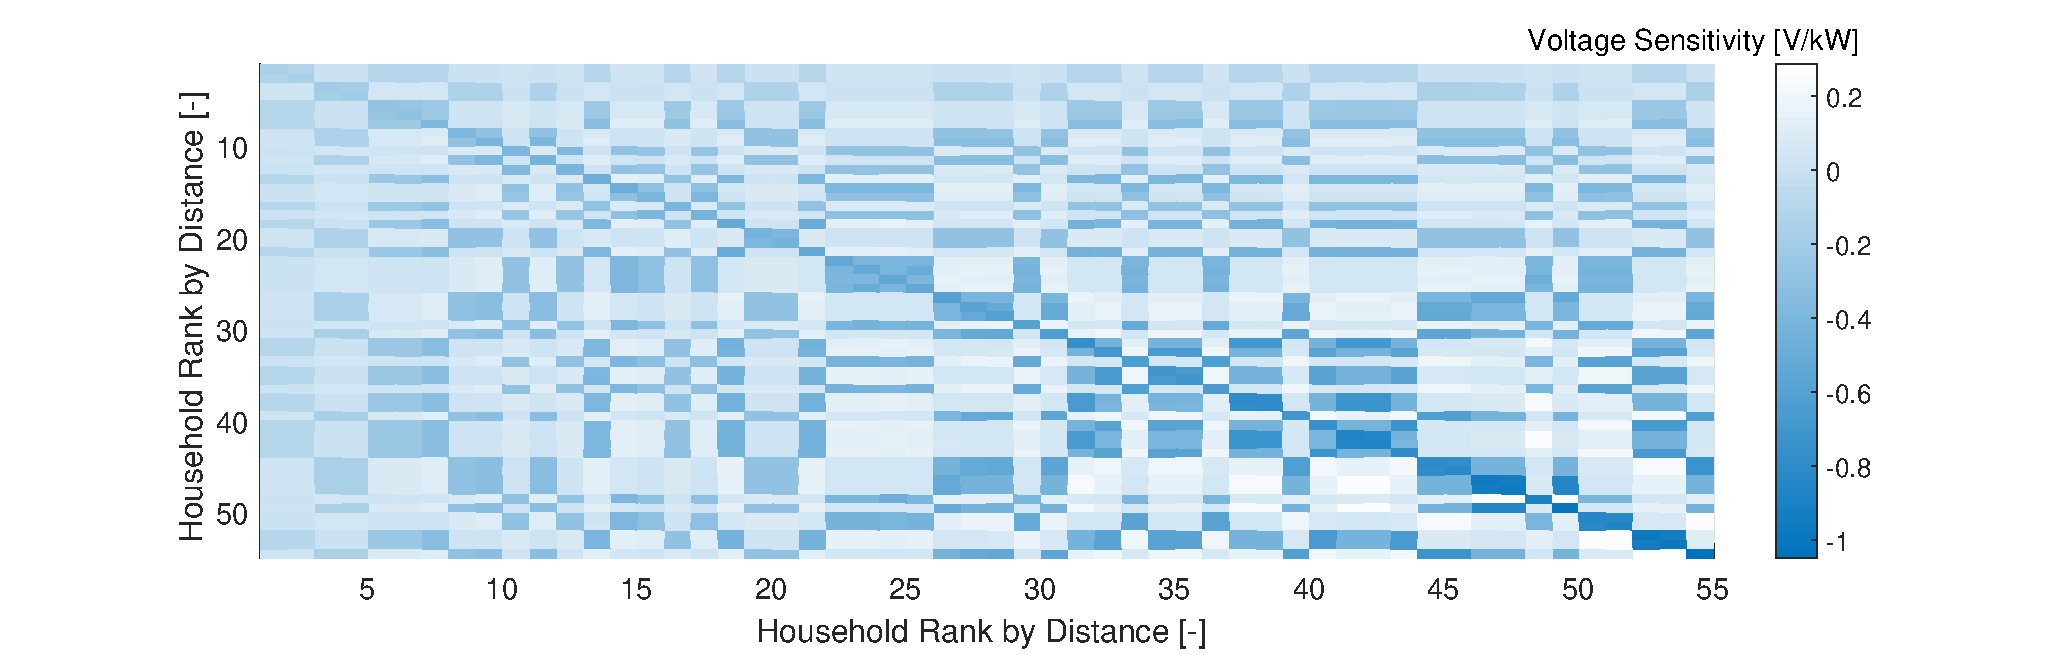
\includegraphics[width=\textwidth,trim={2cm 0cm 2cm 0cm}, clip]{figures/linear/v_sensitivity.eps}
		\label{fig:v_sensitivity}
	}
	\hfill
	\subfloat[Sensitivities of main feeder loading]{
		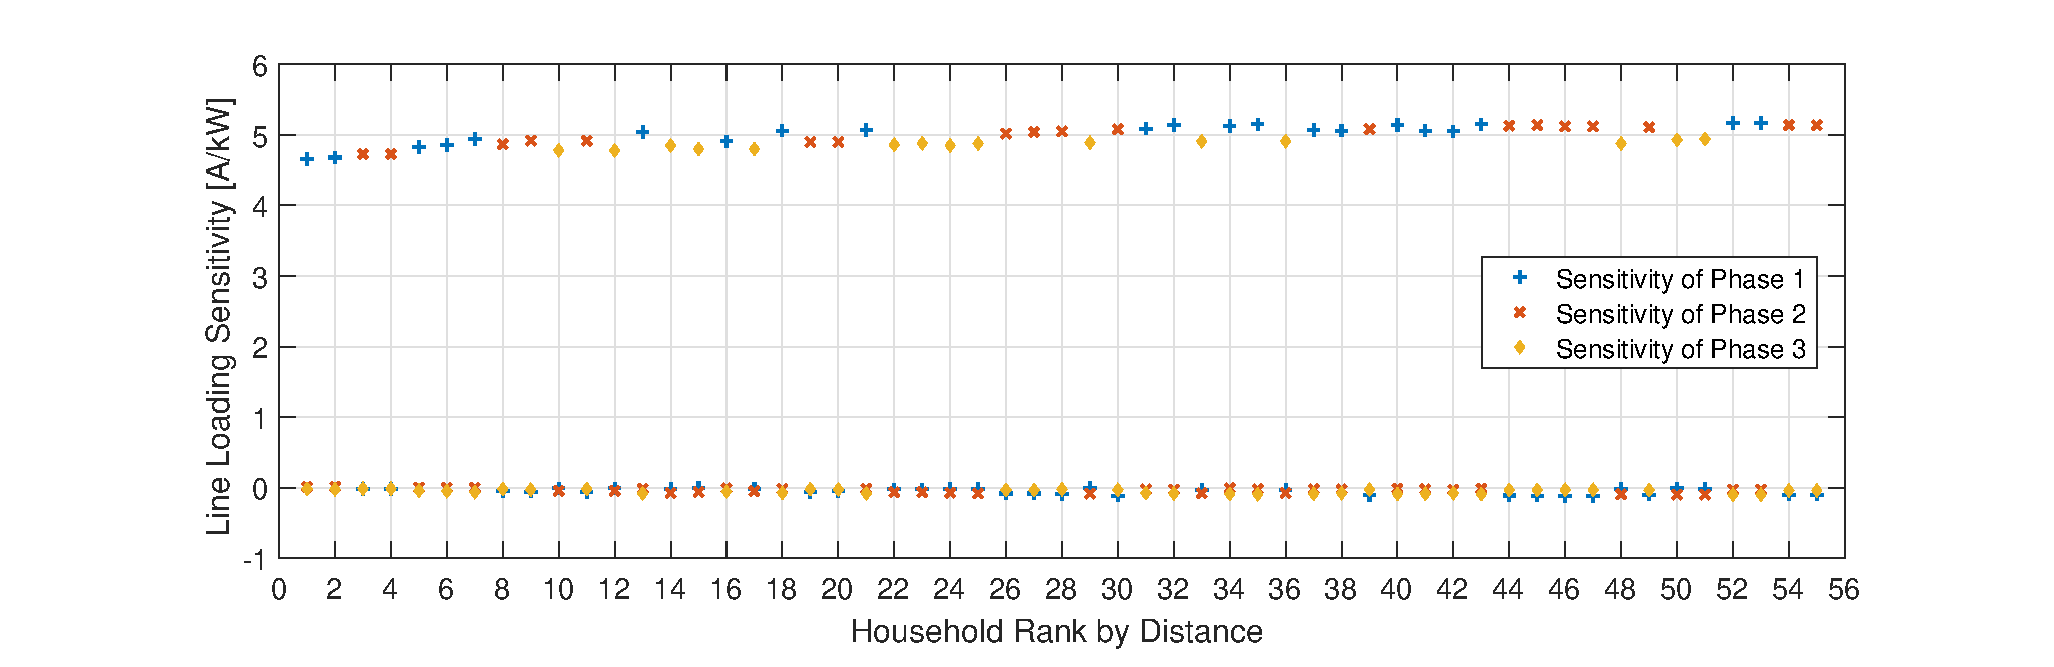
\includegraphics[width=\textwidth,trim={2cm 0cm 2cm 0cm}, clip]{figures/linear/s_sensitivity.eps}
		\label{fig:s_sensitivity}
	}
	\caption{Network sensitivities}
	\label{fig:sensitivities}
\end{figure}

% Describe sensitivity matrices
The sensitivity matrices obtained from this approach are portrayed in \Autoref{fig:sensitivities}. From \Autoref{fig:v_sensitivity} it becomes apparent that voltage drops intensify with increasing distance from the substation and focus on connections close to the location where the load is altered. The magnitude of voltage deviations ranges from -1 V/kW to 0.2 V/kW and protrude when the particular household is connected to the same phase as the point of load variation. The observed increase in phase voltages due to additional load in another phase is not uncommon in unbalanced distribution networks \cite{Richardson2012}. Similarly, the sensitivity of the primary feeder loading portrayed in \Autoref{fig:s_sensitivity} is limited to the phase at which the load is varied. Due to losses and voltage drops along the feeder a slight increase in current sensitivities can be noted with increasing distance from the substation. 

\newpage
% Describe how constraints are reformulated.
Using the voltage sensitivity matrix $\bm{\mu}$, the voltage constraint equations transform to

\begin{equation}
V_{min} \leq V^{bus}_{k,t,init}\left(\hat{D}_{k,t}\right) \;+\; \sum_{j=1}^{K} \bm{\mu}_{j,k} \cdot \pevi \leq V_{max}
\end{equation}

where $V^{bus}_{k,t,init}\left(\hat{D}_{k,t}\right)$ is the voltage resulting at the respective household and time slot due to the predicted residential demand $\hat{D}_{k,t}$ without the presence of EV loads. As this value is not altered by the decision variables, it is pre-determined as a parameter by running OpenDSS nonlinear power flow before the optimisation cycle.

Likewise, the line loading constraints are reformulated applying the line loading sensitivity matrix $\bm{\lambda}$ to each phase $r\in \{1,2,3\}$:

\begin{equation}
I_{\ell,r,t,init}^{line}\left(\hat{D}_{k,t}\right)  \;+\; \sum_{j=1}^{K} \bm{\lambda}_{j,r,\ell} \cdot \pevi \leq I_{\ell}^{max}
\end{equation}

where again $I_{\ell,r,t,init}^{line}\left(\hat{D}_{k,t}\right)$ is the current of the respective line, phase and time slot due to the predicted residential demand $\hat{D}_{k,t}$ without the presence of EV loads. Like the initial household voltages, the line loadings are calculated beforehand as parameters through OpenDSS nonlinear power flow.

% Show validity of approximation

The validity assessment of the approximation is presented in \Autoref{fig:validation_linearPF}. The data is obtained from a simulation of uncontrolled charging (cf.\ \Autoref{sec:dumbcharging}), where vehicles simply start charging upon arrival until their battery is full. The disaggregate voltage errors displayed in \Autoref{fig:voltageerrors} reveals a maximum error of only 0.3\%, prevalent underestimation of actual voltages, and naturally no errors in the absence of EV charging demand.

Additionally, analyses of the average voltage errors per time slot unveil a moderate correlation between the mean error of approximated voltages and the aggregated charging rate (\Autoref{fig:corr_schederror}). Furthermore, they show a divisive correlation between the cumulative voltage error of a household and its electrical distance from the substation (\Autoref{fig:voltageerror_hd}), reiterating the nonlinearity of power flow.

\begin{figure}[]
	\centering
	\subfloat[Disaggregate voltage error matrix]{
		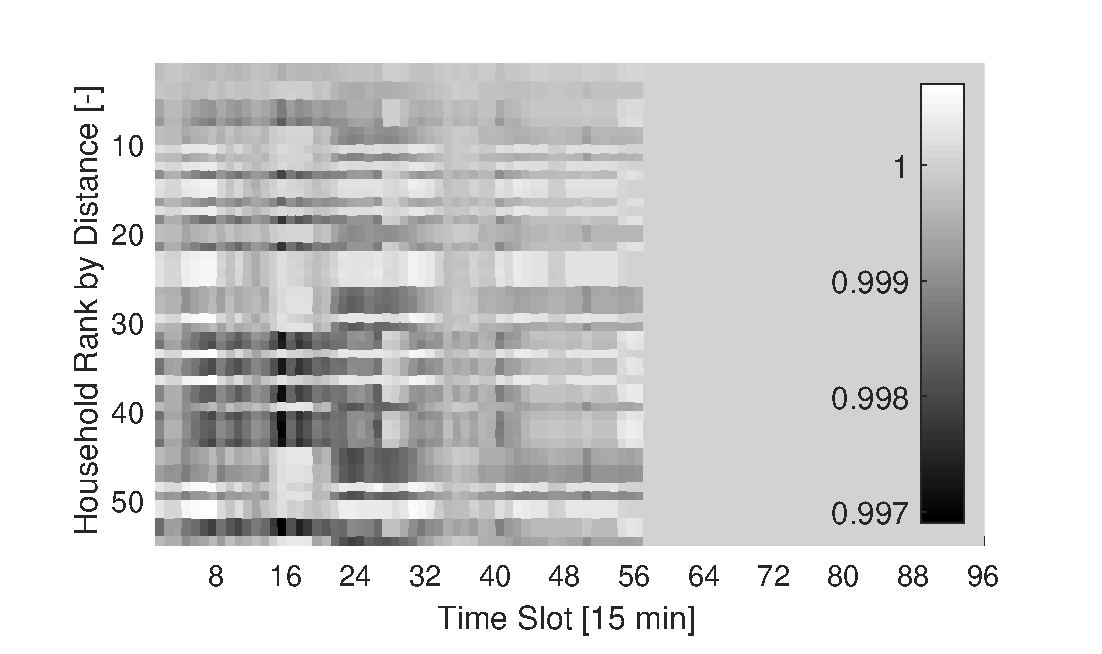
\includegraphics[width=0.48\textwidth,trim={.5cm 0cm .5cm 0cm}, clip]{figures/linear/voltageerrors.eps}
		\label{fig:voltageerrors}
	}
	\subfloat[Line loadings and errors]{
		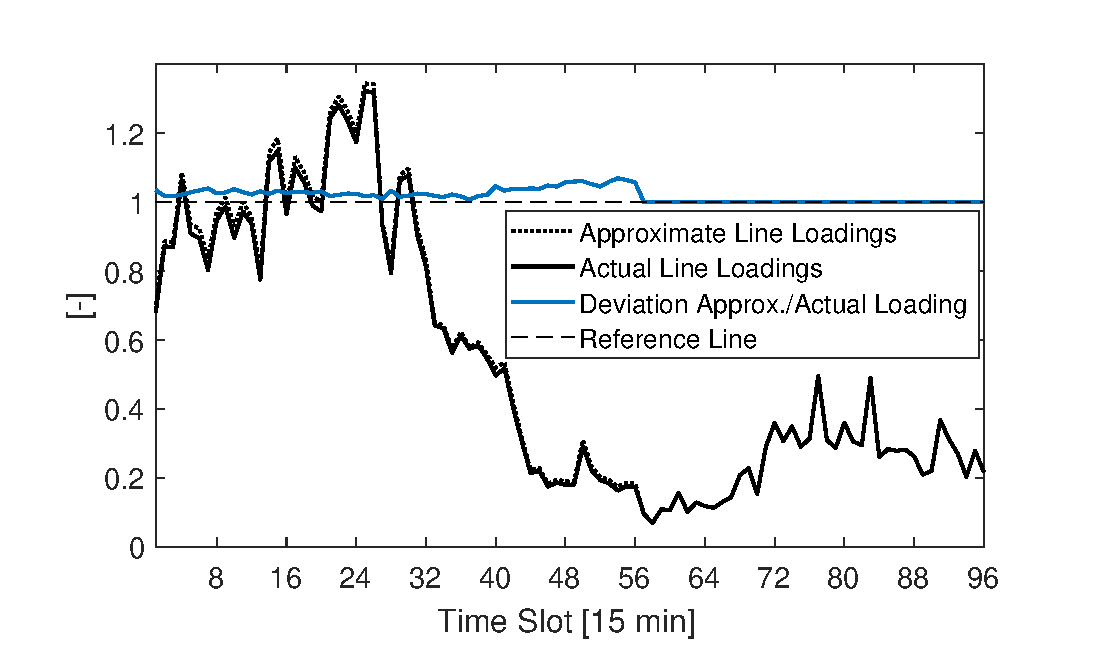
\includegraphics[width=0.48\textwidth,trim={.5cm 0cm .5cm 0cm}, clip]{figures/linear/line_error.eps}
		\label{fig:line_error}
	}
	\hfill
	\subfloat[Correlation between schedule and voltage errors]{
		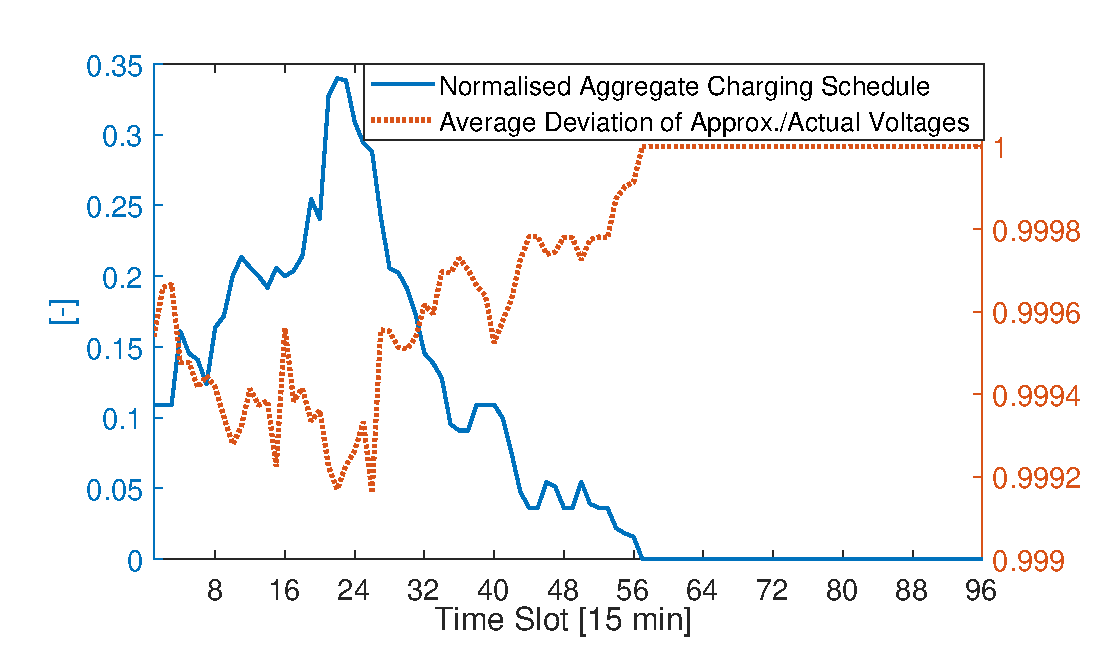
\includegraphics[width=0.48\textwidth,trim={.5cm 0cm .5cm 0cm}, clip]{figures/linear/corr_schederror.eps}
		\label{fig:corr_schederror}
	}
	\subfloat[Cumulative voltage error over time]{
		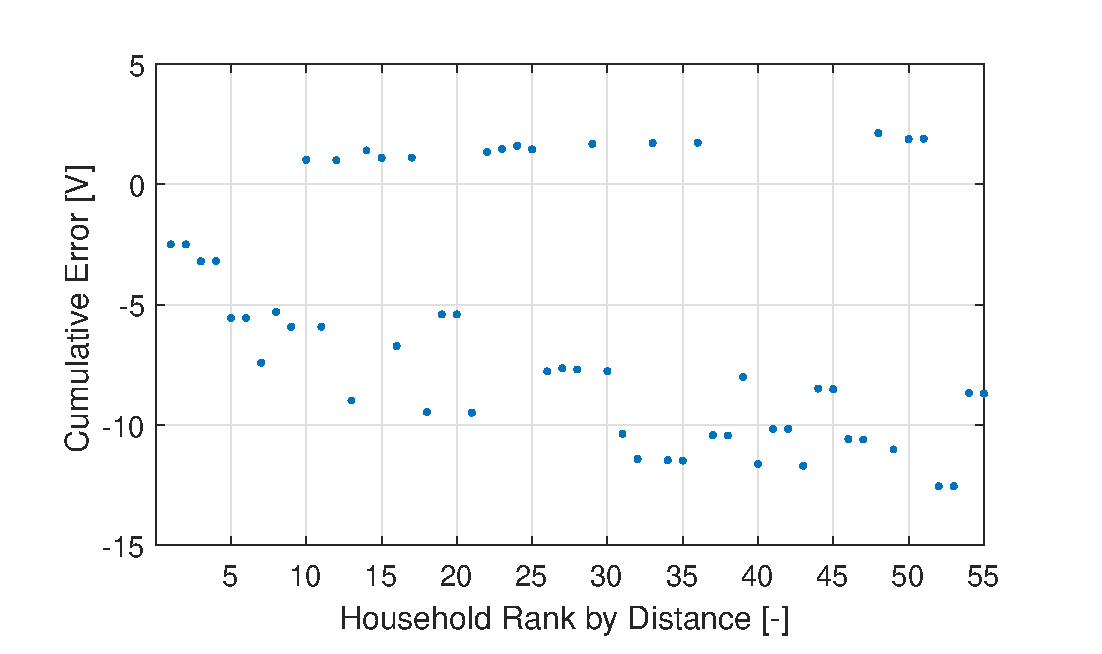
\includegraphics[width=0.48\textwidth,trim={.5cm 0cm .5cm 0cm}, clip]{figures/linear/voltageerror_hd.eps}
		\label{fig:voltageerror_hd}
	}
	\hfill
	\caption{Validation of linear power flow approximation}
	\label{fig:validation_linearPF}
\end{figure}

In line with the voltage approximations, line loadings depicted in \Autoref{fig:line_error} are slightly overestimated throughout the simulation horizon peaking at 6.8\% deviation. Overall, despite small inaccuracies the sensitivity matrices meet the requirements of a conservative approximation and are consistent with expectations, justifying their application. 

\begin{figure}[]
	\includegraphics[width=\textwidth,trim={1.5cm 0cm 2cm 0.2cm},clip]{figures/reference/dumb_ex.eps}
	\caption{Comparison of reference cases: uncontrolled charging and price-based optimisation}
	\label{fig:dumbprice}
\end{figure}

\begin{figure}[]
	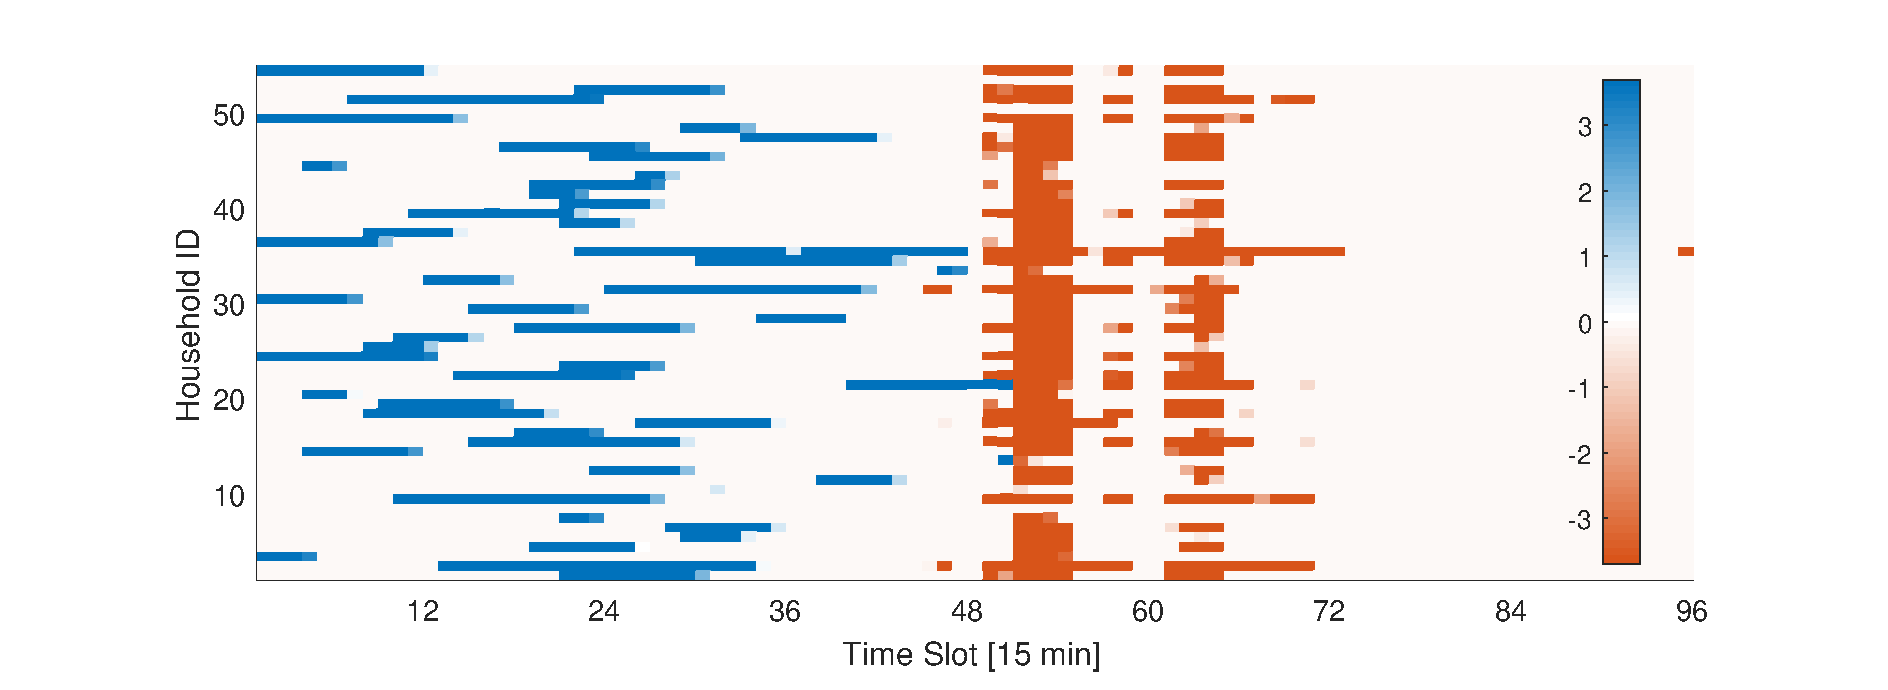
\includegraphics[width=\textwidth,trim={1.5cm 0cm 2cm 0.2cm},clip]{figures/reference/ref_scheds.eps}
	\caption{Comparison of reference cases: schedules (kW/-kW)}
	\label{fig:ref_scheds}
\end{figure}

\section{Reference Charging Approaches}
\label{sec:rc}

Two central reference charging approaches are implemented to assess the performance of the EV scheduling strategies presented in \Autoref{sec:chargecoordination}. The simulation of uncontrolled charging, commonly dubbed `dumb charging', provides a reference case for investigating the economic and technical benefits of charging coordination. Purely price-based optimisation serves as a benchmark for the costs of introducing technical network constraints.

\subsection{Uncoordinated Charging}
\label{sec:dumbcharging}

Uncoordinated charging refers to the situation where no form of control is applied, and EV loads behave as passive loads. It seeks to minimise the time to recharge the battery completely and thereby maximise the driving range available at each time slot. It is a benchmark that commonly complements the evaluation of EV scheduling approaches \cite{GonzalezVaya2015a, Galus2011, Papadopoulos2012, Wu2013, Schuller2013}.

Charging starts directly after grid connection after the last trip of the day and continues at the maximum charging rate until the battery is fully charged unless the vehicle is disconnected prematurely by the user. This `plug and charge' strategy disregards economic incentives to defer EV loads and the network state for its charging decisions.

Charging costs are evaluated based on two scenarios. First, the aggregator is obliged to purchase the inflexible aggregate demand in the market and passes the cost determined by the price time series $\pi$ on to the customers \cite{GonzalezVaya2015a}. Second, the average price $\bar{\pi}$ emulates a single-rate tariff offered by the energy utility for static loads. The latter case mirrors best the benefit an EV user would have from switching from a conventional single-rate electricity tariff to a contract with a coordinating aggregator with access to the wholesale market.

The general impact of uncontrolled EV loads has been investigated in multiple studies as summarised in  \Autoref{sec:impact}. A run of uncontrolled charging in the built model matches the analyses of previous work: \Autoref{fig:dumbprice} exposes that EV charging is centred upon periods of high residential demand, thereby causing occasional overloads and voltage violations when the aggregate of residential and EV load peaks. The coincidence of EV loads with high spot prices makes uncontrolled charging a liability for the grid integration of renewable energy sources.

\subsection{Price-Based Optimisation}
\label{sec:pbh}

A purely price-based heuristic scheduling approach serves as a reference optimisation, first, to illustrate the need for coordination of EV charging processes when access to the wholesale market is granted and, second, to quantify the cost of applying network constraints.

The scheme the heuristic follows is outlined in Algorithm \ref{alg:price}. Electricity prices are initially sorted in ascending order from lowest to highest values, and a charging schedule is determined independently for each electric vehicle. No coordination between EVs takes place, and schedules can be achieved without information exchange to a third-party agent. Among the slots in which a particular vehicle is plugged in, starting with the cheapest slot charging rates are set to their maximum in the next cheapest slot until the battery is completely charged.

\begin{algorithm} 
	\caption{Price-based Heuristic Scheduling}
	\begin{spacing}{1.2}
		\begin{algorithmic}[1]
			%\Require $\pi\in\mathbb{R}^T$, the simulated price time series
			\State Sort prices $\pi\in\mathbb{R}^T$ in ascending order $\sigma \in \mathbb{N}^T$
			\State Initialise empty vehicle charge schedules: $P^{EV} = \bm{0}_{K,T}$
			\ForEach {household $k \in K $}
			\State {Determine vehicle energy demand: $D^{EV}_k \gets B_{max} - B^{arr}_k$}
			\ForEach {time slot $t \in T $}
			\While {$D^{EV}_k > 0$}
			\If{$\alpha^{EV}_{k,\sigma(t)} = 1$}
			\State {$P^{EV}_{k,\sigma(t)} \gets \min\left\{P_{max}, \frac{D^{EV}_k}{\eta \cdot \Delta t}\right\}$}
			\State {$D^{EV}_k \gets D^{EV}_k - P^{EV}_{k,\sigma(t)} \cdot \eta \cdot \Delta t$}
			\EndIf
			\EndWhile
			\EndFor
			\EndFor
			\State \Return {complete vehicle charge schedules: $P^{EV}\in \mathbb{R}^{K\times T}$}
		\end{algorithmic}
	\end{spacing}
	
	\label{alg:price}
\end{algorithm}

This greedy heuristic, when applied with perfect forecasts, produces a schedule causing the least charging costs possible to satisfy user demands given the EV availability periods. Because prices may be the same in multiple time slots, different optimal schedules are conceivable but would ultimately result in the same minimal charging costs for the given model. These costs are a lower bound against which any charging costs obtained by algorithms considering additional constraints (e.g.\ concerning network state or conservation of EV batteries) can be assessed.

The comparison with the uncontrolled charging approach in \Autoref{fig:dumbprice} reveals a tendency for high concentration of loads in cheap time slots. This is because every EV agent is assumed to act rationally towards her maximum economic benefit and low prices happen to intersect with the availability periods of EVs. In comparison to uncontrolled charging, this may lead to even more severe voltage violations and mains cable overloading. Consequently, without local adaptation of electricity prices to reflect the state of the low-voltage distribution network by means such as locational marginal pricing (LMP), purely price-based charging might balance the volatility of renewable generation and electricity demand but not foster high capacity exploitation and load accommodation in distribution networks. New load peaks due to low price signals in distributed optimisation may be alleviated by applying physical constraints.

\section{Charge Rate Coordinating Scheduling Methods}
\label{sec:chargecoordination}

%Explain need for coordination

Evidently, both uncontrolled EV charging and price-based heuristic scheduling fail to observe statutory voltage limits and thermal line ratings at all times and are inept to guarantee a safe network operation. However, the dual role of the aggregator not only entails a commitment to the economic benefit and demand satisfaction of individual consumers but also the technical requirements of the distribution network operator. While the two reference cases excel at reliably re-charging batteries, by violating network constraints the aggregator puts its obligation to the distribution system operator in second place. Thus, two methods incorporating system constraints were developed: a linear program and a heuristic optimisation extending upon the price-based reference methods. 

\subsection{Linear Programming}

Thanks to the linear power flow approximation through network sensitivities introduced in \Autoref{sec:lpf} the EV scheduling problem can be easily and quickly solved by a linear program. In this work, Gurobi is used as a solver and embedded in the simulation framework. Except for the limitations induced by possible prediction errors and the linear power flow approximation, the solver will produce the best coordination of EV charging processes regarding both \textit{when} and \textit{which} EVs should charge. Due to the centralised approach to scheduling, it requires significant information exchange of input parameters between customer and aggregator and likely entails poor scalability.

\subsection{Network-Constrained Price-Based Heuristic Optimisation}

Other than the centrally organised linear program, in the extended price-based heuristic (\Autoref{sec:pbh}) cost-minimising schedules are determined locally without prior knowledge of the network conditions and submitted to the aggregator. Subsequently, the aggregator checks whether the new schedule in addition to previously committed schedules and demand forecasts causes any voltage issues or exceeds network capacities. If violations occur, the aggregator rejects the schedule and imposes a suitable load limitation signal according to which the vehicle is rescheduled locally. Otherwise, the schedule is adopted, and the aggregator awaits the schedule proposal of the next electric vehicle. This process is repeated iteratively until all electric vehicles are scheduled. Full insight into the functioning principle of the heuristic is provided in Algorithm \ref{alg:ncpbh}.

Because the order by which EV schedules are taken influences the performance of the heuristic, several cases are examined where the priority list $\theta \in \mathbb{N}^K$ is determined

\begin{itemize}
	\item by EV arrival time in ascending order,
	\item by EV availability period in ascending order,
	\item by EV battery state of charge upon arrival in ascending order,
	\item by electrical distance of household from substation in ascending order, or
	\item by electrical distance of household from substation in descending order.
\end{itemize}

Prioritising by \textit{arrival time} constitutes an easy escape from arrival and battery state of charge uncertainty if power can be traded on an intraday market and schedules are proposed and checked by the aggregator upon arrival in real time.

Sorting by the expected \textit{availability period} or the \textit{initial battery state of charge} of an electric vehicle ranks the vehicles by their degree of load flexibility. It avoids that an inflexible electric vehicle cannot be fully loaded because all its charging options are exhausted as limits in the network are reached. The primary motive is to achieve a high demand satisfaction rate.

Sorting by \textit{ascending electrical distance} aims at accommodating the maximum amount of EVs in inexpensive time slots. This makes use of the observation that due to the radial layout of the distribution network voltage levels are less sensitive to the addition of loads near the substation \cite{Richardson2012}. Conversely, A priority list based on \textit{descending electrical distance} should expose significantly lower energy delivery in the cheapest slots. This approach makes price reduction a priority and might result in electric vehicles at the end of the feeder paying higher rates for charging due to load limitation signals in already fully exploited inexpensive slots. This inequality would require a fair cost redistribution through the aggregator.
 
\begin{algorithm}[h]
	\caption{Network- and Price-Based Heuristic Scheduling}
	\label{alg:ncpbh}
	\begin{spacing}{1.2}
	\begin{algorithmic}[1]
		%\Require $\pi\in\mathbb{R}^T$, the simulated price time series
		\State Sort prices $\hat{\pi}\in\mathbb{R}^T$ in ascending order $\sigma \in \mathbb{N}^T$
		\State Determine order $\theta\in  \mathbb{N}^K$ by which vehicles are scheduled
		\State Initialise empty vehicle charge schedules: $P^{EV} = \bm{0}_{K,T}$
		\ForEach {household $k \in K$}
		\State {Determine vehicle energy demand: $D^{EV}_{\theta(k)} \gets B_{max} - B^{arr}_{\theta(k)}$}
		\State {Initialise set of charging rate limits induced by network state: $P_{max}'= (P_{max})_{K,T}$}

		
		\While {$\neg\forall \ell\in L, t\in T, k\in K\; V_{min} \leq V_{k,t}^{bus} \leq V_{max} \text{ and } I_{\ell,p,t}^{line} \leq I_{\ell}^{max}$}
		\ForEach {time slot $t \in T $} %\Comment{Calculate greedy schedule proposal}
		\While {$D^{EV}_{\theta(k)} > 0$}
		\If{$\alpha^{EV}_{{\theta(k)},\sigma(t)} = 1$}
		\State {$P^{EV}_{{\theta(k)},\sigma(t)} \gets \min\left\{P_{max}, \frac{D^{EV}_{\theta(k)}}{\eta \cdot \Delta t}\right\}$}
		\State {$D^{EV}_{\theta(k)} \gets D^{EV}_{\theta(k)} - P^{EV}_{{\theta(k)},\sigma(t)} \cdot \eta \cdot \Delta t$}
		\EndIf
		\EndWhile
		\EndFor
		
		%\Comment{Check proposed schedule for infeasibilities and mitigate}
				
		\If {$\neg\forall \ell\in L, t\in T, k\in K:\; V_{min} \leq V_{k,t}^{bus} \leq V_{max} \text{ and } I_{\ell,p,t}^{line} \leq I_{\ell}^{max}$}
		\State Find set of slots $T_{viol}\subset T$ with technical violations
		\ForEach {$\tau \in T_{viol}$}
		\State {$P_{max,\theta(k),\tau}' \gets P^{EV}_{\theta(k),\tau}-\Delta P$} \Comment {$\Delta P$ denotes step size of load limitation}
		\If {$P_{max,\theta(k),\tau}' \leq 0$}
		\State {$\hat{\pi}_\tau \gets \infty$}
		\EndIf
		\EndFor
		\State Re-sort prices $\hat{\pi}\in\mathbb{R}^T$ in ascending order $\sigma \in \mathbb{N}^T$
		\State Reset schedule: $P^{EV}_{{\theta(k)},\sigma(t)} \gets 0$ for all $t \in T$
		\EndIf
		
		\EndWhile
		

		\EndFor
		\State \Return {complete vehicle charge schedules: $P^{EV}\in \mathbb{R}^{K\times T}$}
	\end{algorithmic}
	\end{spacing}
	\label{alg:network}
\end{algorithm}

Other than the linear program, the network-constrained heuristic does not require a linear power flow approximation but can retrieve accurate voltage and line loading measurements directly from the OpenDSS simulation. Moreover, it constitutes a slightly more decentralised approach involving less information exchange improving privacy preservation and scaling-induced complexity because schedule proposals are now determined locally, and the aggregator only monitors the status of the distribution network. Due to the lack of formality in heuristic optimisation, there is no guarantee for an optimal solution. Nevertheless, the evaluation of priority lists will support the understanding of the primary determinants affecting the optimal charging coordination of electric vehicles, which the linear program lacks to illustrate.

\section{Approaches to Uncertainty Mitigation}
\label{sec:uncmitigation}

% uncertainties involved and assumptions

Because EV charging coordination is embedded in a highly stochastic environment but most decisions may have to be taken before observing realisations of uncertain parameters, optimisation based solely on expectation values is not robust and offers potential to extenuate sensitivities towards forecast deviations. Consequently, this section introduces uncertainty mitigation options which are subsequently evaluated in \Autoref{sec:saunc}. Note that the presented concepts rely on the assumption that based on the empirical data of a user, probabilities for input parameters can be defined similarly to the modelled distribution functions, conscious that this was yet another modelling approximation. 

Classical \textit{robust optimisation} is a method for risk-averse decision making yielding the least worse outcome. It is commonly applied when parameters are known only within certain bounds, and uncertainty preponderates in constraints. Its primary goal is to find undoubtedly feasible solutions, whereas optimisation is just the secondary objective. The high level of conservatism involved may incur substantial cost increases \cite{Bertsimas2004}. 

Quantifying the uncertainty in the true value of a parameter by empirical or idealised probability distributions allows \textit{stochastic programming}. This method requires much more insight into historical consumption patterns and extends robust optimisation \cite{Sim2017}. Other than robust optimisation, however, its goal is to find an optimal solution that is feasible for almost all possible parameter sets, relaxing the usually expensive worst case consideration. For heavily interwoven uncertainties, where the interlink between parameters is unknown, it is common to reduce complexity via a scenario tree by extracting at random some instances of the uncertain parameters and find a feasible solution for these samples. For the scheduling of electric vehicles, the adversity of parameter uncertainties can largely be quantified and identified separately, so that individual security margins for unfavourable cases of a particular parameter can be defined. Although no financial weighting between constraint satisfaction and cost minimisation is assumed, applied security margins provide the ability to mimic appropriate weightings. Further, it should be noted despite attempting to mitigate uncertainty, the optimisation routine is deterministic and recognises the stochasticity of the problem by adapting its input parameters only according to the pre-calculated probability distributions.

% TODO check and cite some things

\subsection{Availability Uncertainty}
\label{sec:av_unc}

Uncertainty about the arrival and departure times of electric vehicles can be defused using the historical mobility profile of an EV owner. Instead of using the expectation values as forecasts, $\hat{\alpha}^{EV}_{t}$ may indicate time slots in which the availability probability $\mathbb{P}\left(\alpha_t^{EV}=1\right)$ is larger than a given threshold. As outlined in \Autoref{sec:mub}, the availability probability is calculated from the CDFs of the arrival and departure time distributions and is illustrated in \Autoref{fig:av_mit}. While choosing a high threshold demanding a degree of certainty of $\nu_{\alpha}$ reduces charging flexibility by narrowing the predicted availability period, it also reduces the chances of an electric vehicle scheduled to charge in times where it is not available. At the cost of missing cheap slots where the car actually turns out to arrive earlier or depart later than predicted, the robustness to forecast deviations is increased in terms of fulfilling customer demand for a full battery. Thus,

\begin{equation}
\hat{\alpha}'^{EV}_{t} = \begin{cases}
1 & \text{if  }\mathbb{P}\left(\alpha^{EV}_{t}=1\right) \geq \nu_{\alpha} \\
0 & \text{else}
\end{cases}
\end{equation}

% An alternative to (penalty) defines the cost of 

\begin{figure}[]
	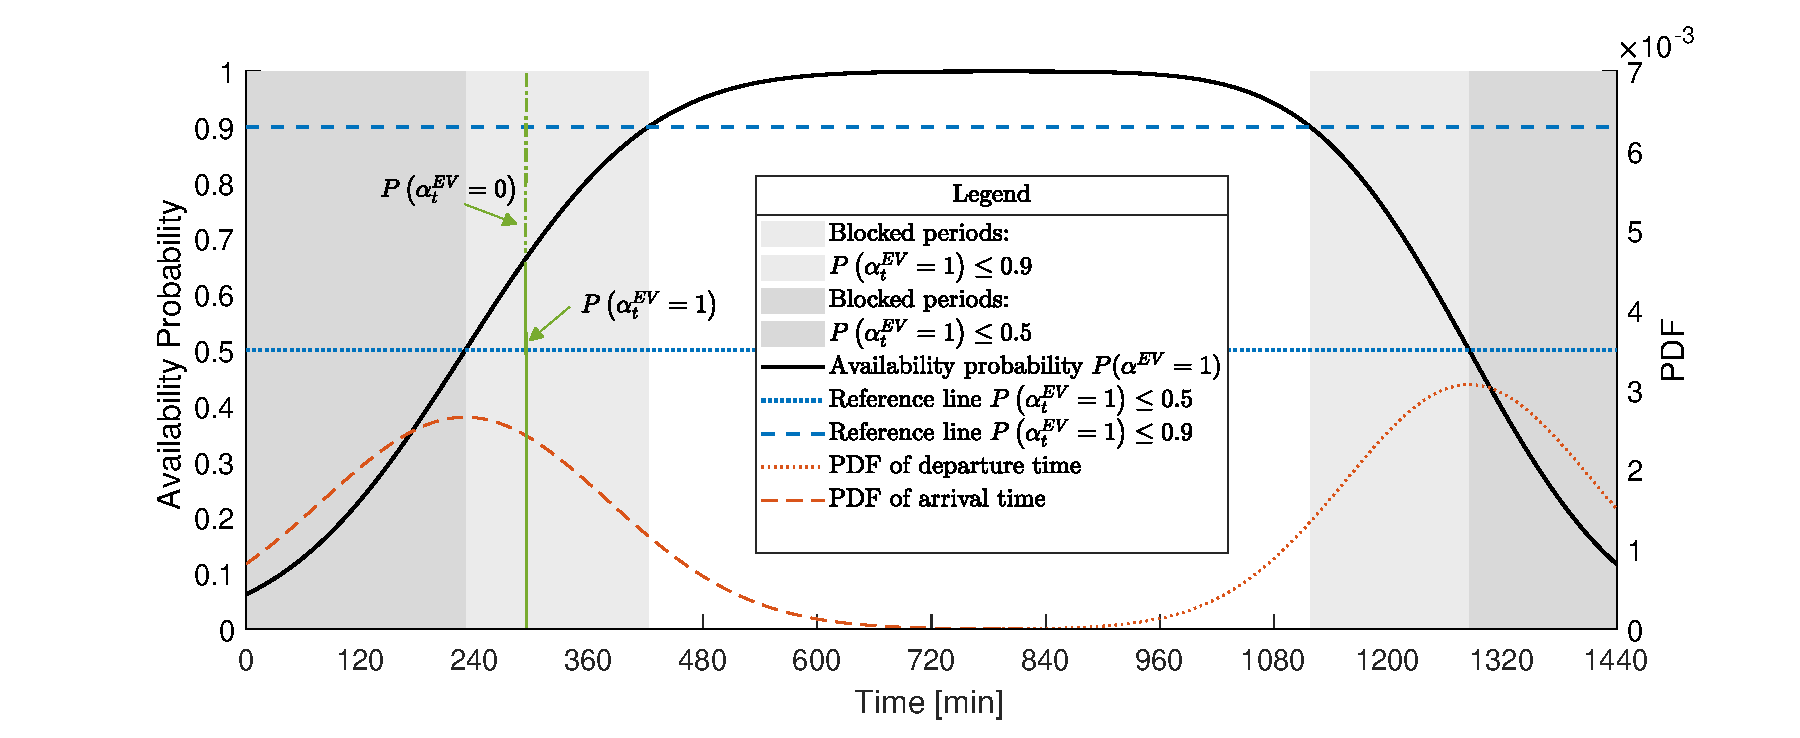
\includegraphics[width=\textwidth,trim={1.5cm 0cm 1.5cm 0.2cm},clip]{figures/mitigation/av_mit.eps}
	\caption{Approaches for the mitigation of availability uncertainty}
	\label{fig:av_mit}
\end{figure}

\subsection{Battery Charge Level Uncertainty}

Uncertainty mitigation concerning the battery state of charge upon arrival in day-ahead scheduling is likewise rested on historical mobility profiles of individual EV users. Deviation from the maximum likelihood estimator as a forecast value $\hat{B}^{arr}$ involves a trade-off between the risk of not fully charging a battery if the SOC is less than predicted and excessive scheduling if the SOC is higher than expected for robustness, thereby blocking eventually fallow network capacity. The issue is depicted in \Autoref{fig:soc_mit}. Assuming a state of charge exceeded in a ratio of $\nu_{B}=0.7$ of all cases instead of its actual expectation value will increase the likelihood of curtailment due to a full battery achieved prematurely. Prioritising customer satisfaction over reduced capacity and price exploitation, sensitivity analysis in \Autoref{sec:saunc} focusses on the cost of excessive scheduling.

\begin{figure}[]
	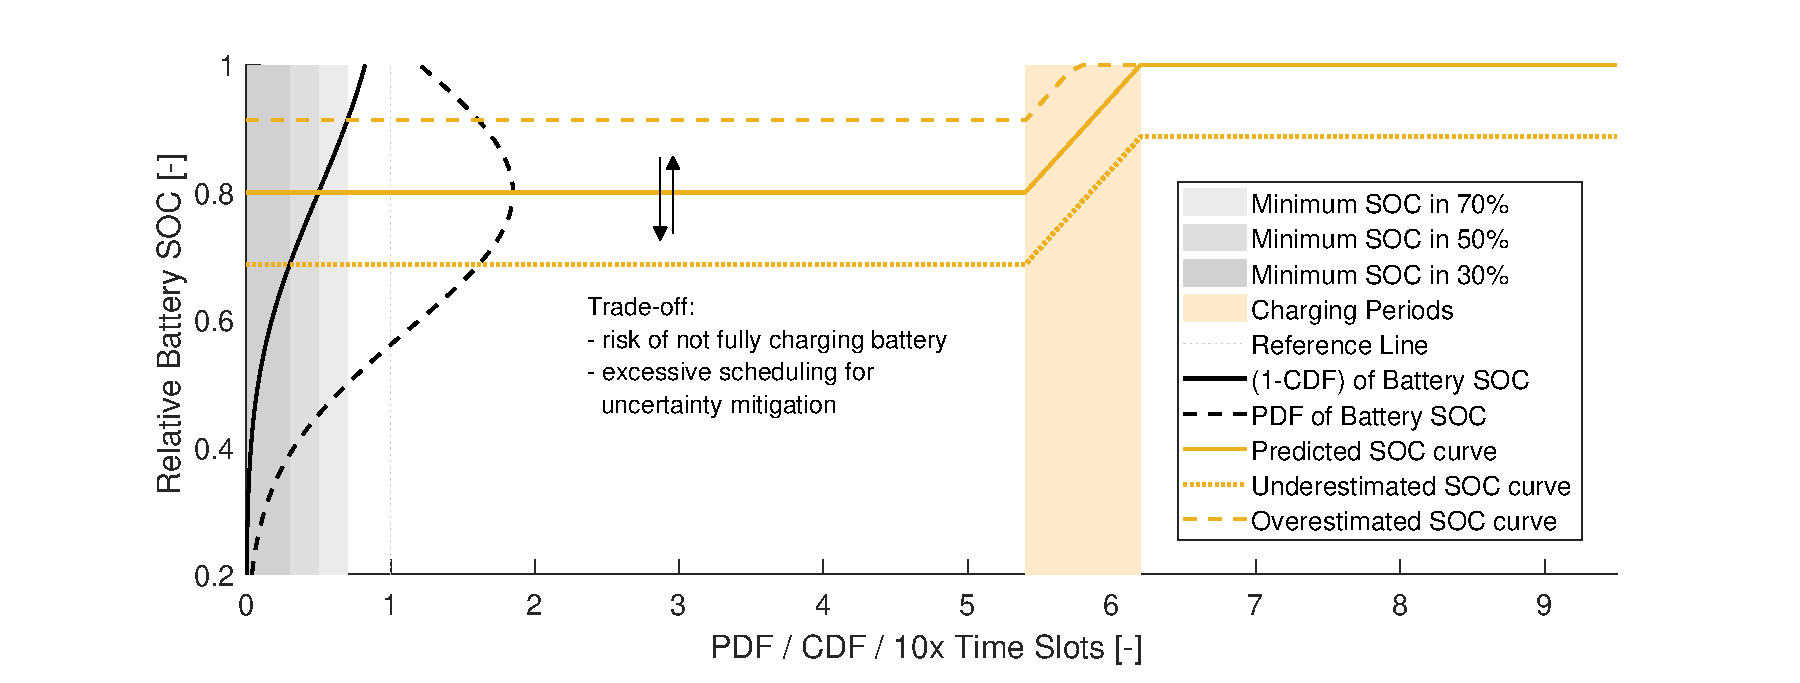
\includegraphics[width=\textwidth,trim={2.1cm 0cm 2.1cm 0.2cm},clip]{figures/mitigation/soc_mit.eps}
	\caption{Mitigation of battery state of charge uncertainty}
	\label{fig:soc_mit}
\end{figure}

\subsection{Spot Price Uncertainty}

Mitigation of price uncertainties relies on the assumption that forecasts can be given with certain error margins and distributions. Furthermore, it is clear that uncertainty of price time series is only relevant if the ranking is distorted significantly and hedging against severe underestimation of prices is a priority for risk-averse aggregators. Instead, expectation values could be replaced by their $\nu_{\pi}$-quantiles as the price input for each time slot. This quantile refers to the rate which is not exceeded in $100\cdot\nu_{\pi}$ \% of cases. Although this input deviates from the best estimator for electricity prices, it reflects the extent of involved uncertainties by deferring highly uncertain time slots to rearward positions in the price ranking. Thereby, it disincentivises a scheduling algorithm to charge in cheap but uncertain slots and increases the robustness of the schedules against adverse realisations of electricity prices. 

For the exemplary price profile of \Autoref{sec:pr_unc}, \Autoref{fig:pr_mit} visualises the quantiles and ranking distortion compared to the 0.5-quantile. Approximating the worst-case scenario, the ranking distortion measured by the Spearman's rank correlation coefficient intensifies. Nonetheless, the correlation coefficients also expose very limited variation in the ranking. Per design, the cost of mitigation arises from the diminished opportunity to exploit low prices in uncertain time slots.

\begin{figure}[]
	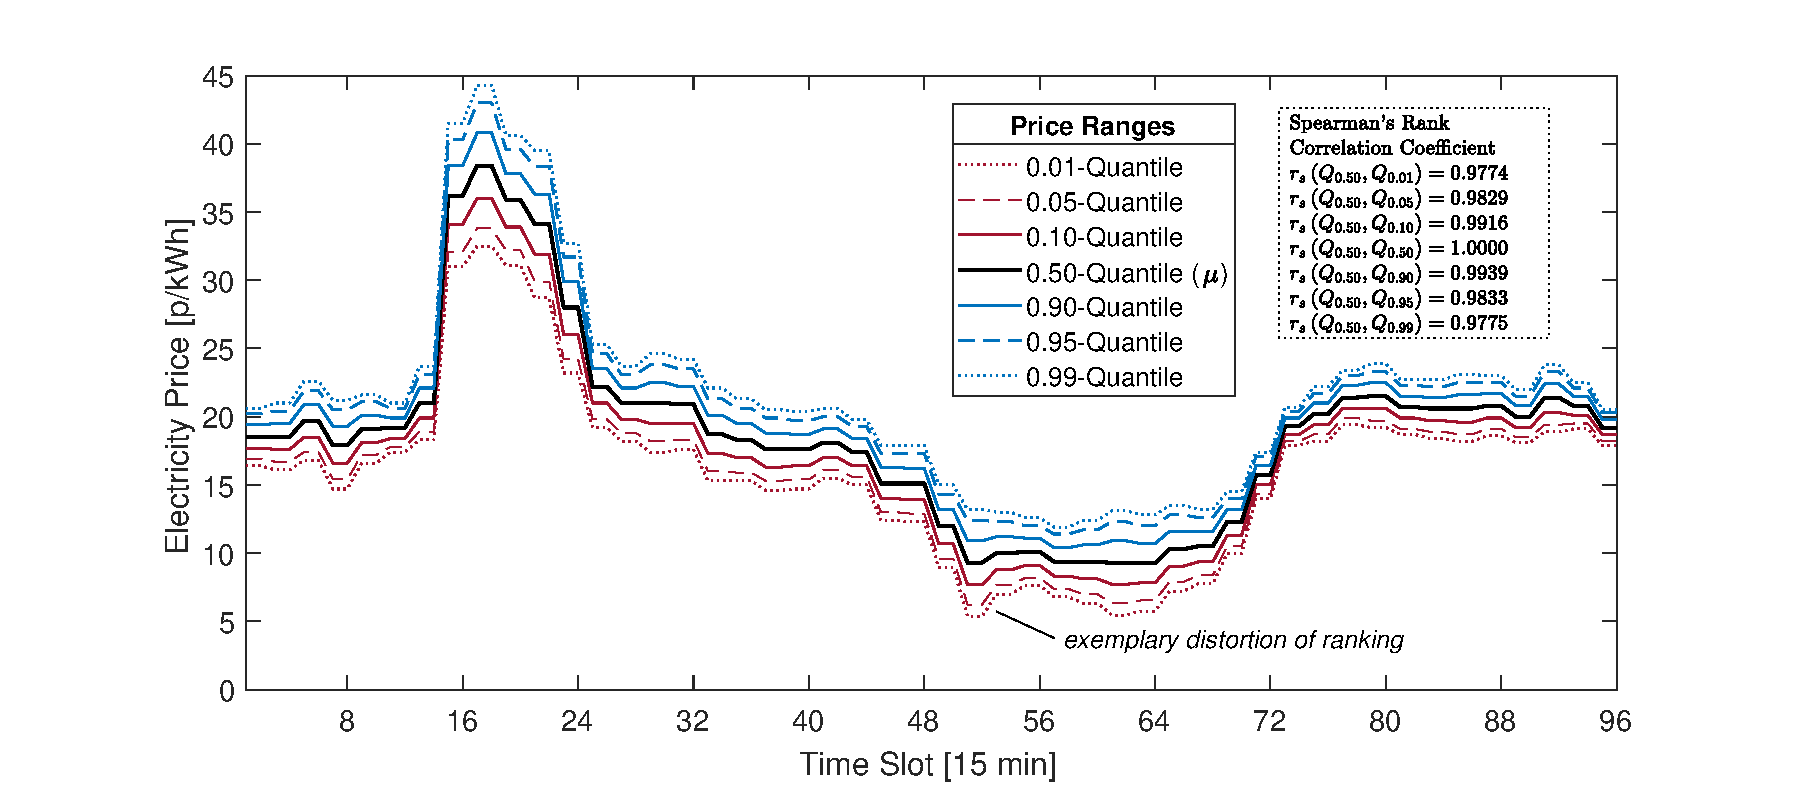
\includegraphics[width=\textwidth,trim={2.1cm 0cm 2.1cm 0.2cm},clip]{figures/mitigation/pr_mit.eps}
	\caption{Approaches to mitigation of price uncertainties}
	\label{fig:pr_mit}
\end{figure}

\subsection{Residential Demand Uncertainty}

In \Autoref{sec:rd_unc} it has been discussed that uncertainty \textit{when} dominates uncertainty about \textit{what} residential demand peaks occur and demand profiles may randomly shift within a certain time frame. Robustness against demand uncertainty is achieved by building a rolling maximum from expected residential loads to form the new demand forecast

\begin{equation}
\hat{D}_t' = \max \left\{\hat{D}_i \;|\; i \in \{t-w_{max},\dots,t,\dots,t+w_{max}\}\right\},
\end{equation}

where $w_{max}$ is the presumed maximum deviation between predicted and simulated demand. Set to 30 minutes in either direction, the adapted residential demand output compares to the prediction as shown in in \Autoref{fig:dem_mit}. This protects the schedule from causing overloads and voltage problems due to residential loads deviating within the window size by anticipating their occurrence in any possible slot. As this approach reduces the available capacity for EV charging, cost increases are foreseen. 

\begin{figure}[]
	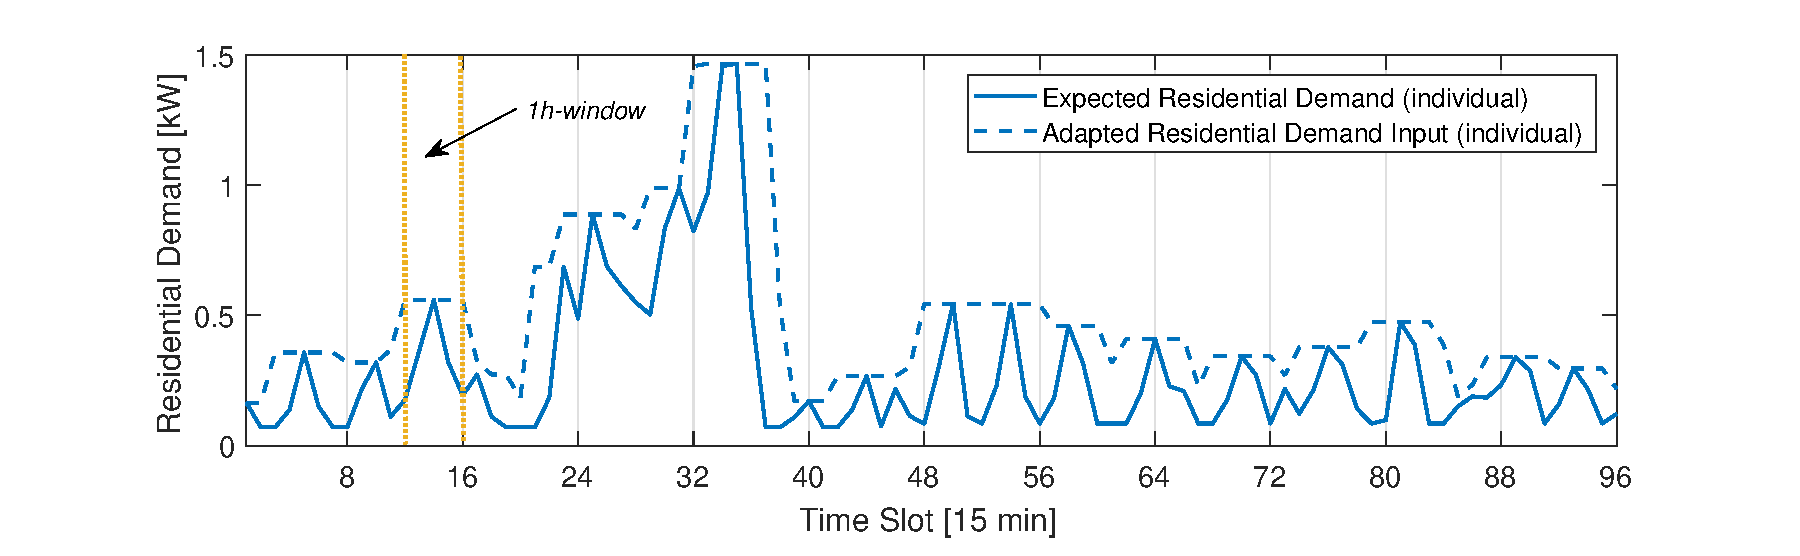
\includegraphics[width=\textwidth,trim={2.1cm 0cm 2.1cm 0.2cm},clip]{figures/mitigation/dem_mit.eps}
	\caption{Illustration of demand uncertainty mitigation}
	\label{fig:dem_mit}
\end{figure}